\documentclass[12pt,a4paper]{article}
\usepackage{physics}
\usepackage{amssymb}
\usepackage{subcaption}
\usepackage{colortbl}
\input{spp.dat}

%  Editorial staff will uncomment the next line
% \providecommand{\artnum}[0]{XX-XX}
% \renewcommand{\articlenum}[0]{SPP-\the\year-\artnum-}

\begin{document}

\title{\TitleFont Activity 4 -- Measuring Area from Images}
\author[ ]{\textbf{Kenneth V. Domingo} \\
2015--03116 \\
App Physics 186, 1\textsuperscript{st} Semester, A.Y. 2019--20}
\affil[ ]{\corremail{kvdomingo@up.edu.ph} }

\maketitle
\thispagestyle{titlestyle}

\section*{Results and Discussion}
\setcounter{section}{1}

For this activity, I generated the basic shapes using the Python Imaging Library (\texttt{PIL}). This let me define the centroid and pseudo-radius (distance from the centroid to a corner) for each shape analytically, and therefore, I know precisely what their dimensions and areas will be. The shapes are shown in Fig. \ref{fig:shapes}, all with size $1024 \times 1024$.

\begin{figure}[htb]
    \centering
	\begin{subfigure}[h!]{0.24\textwidth}
		\centering
		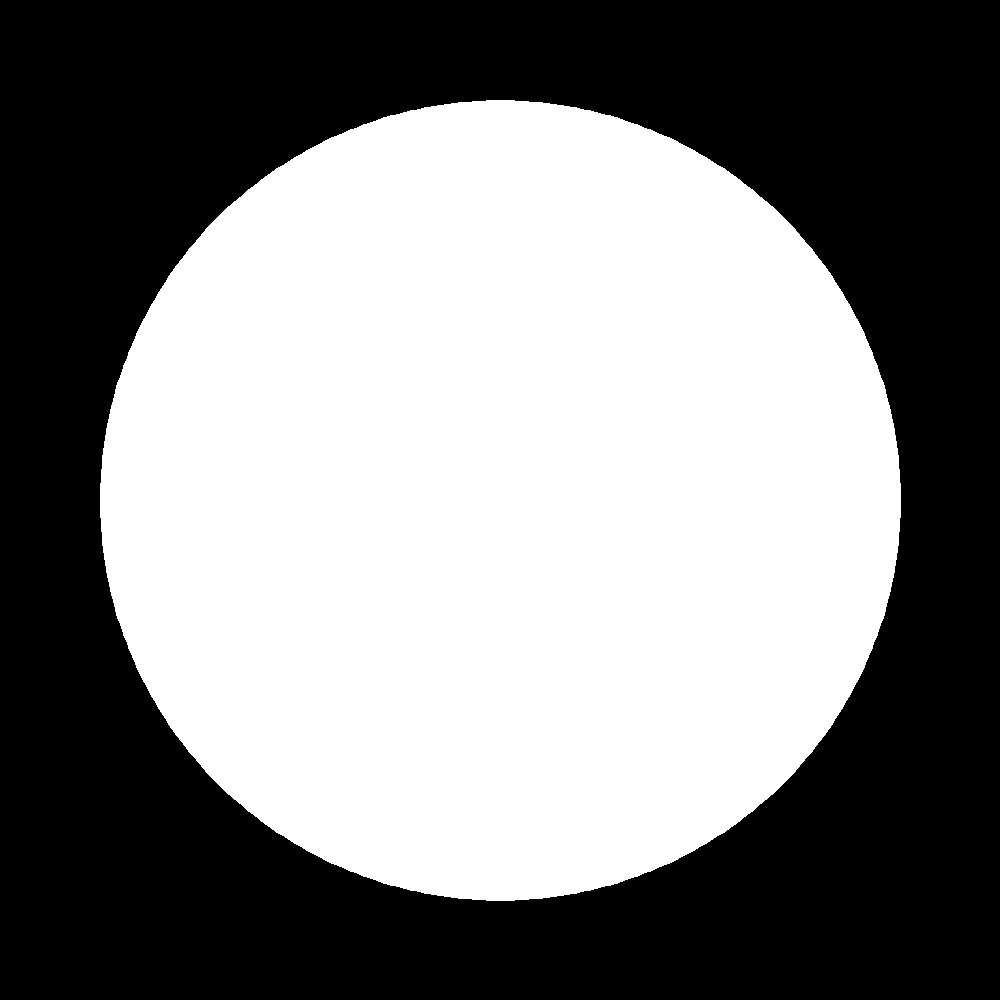
\includegraphics[width=\textwidth]{circle.png}
		\caption{circle}
		\label{fig:circle}
	\end{subfigure}
	\begin{subfigure}[h!]{0.24\textwidth}
		\centering
		
\includegraphics[width=\textwidth]{square.png}
		\caption{square}
		\label{fig:square}
	\end{subfigure}
	\begin{subfigure}[h!]{0.24\textwidth}
		\centering
		
\includegraphics[width=\textwidth]{trapezoid.png}
		\caption{trapezoid}
		\label{fig:trapezoid}
	\end{subfigure}
	\begin{subfigure}[h!]{0.24\textwidth}
		\centering
		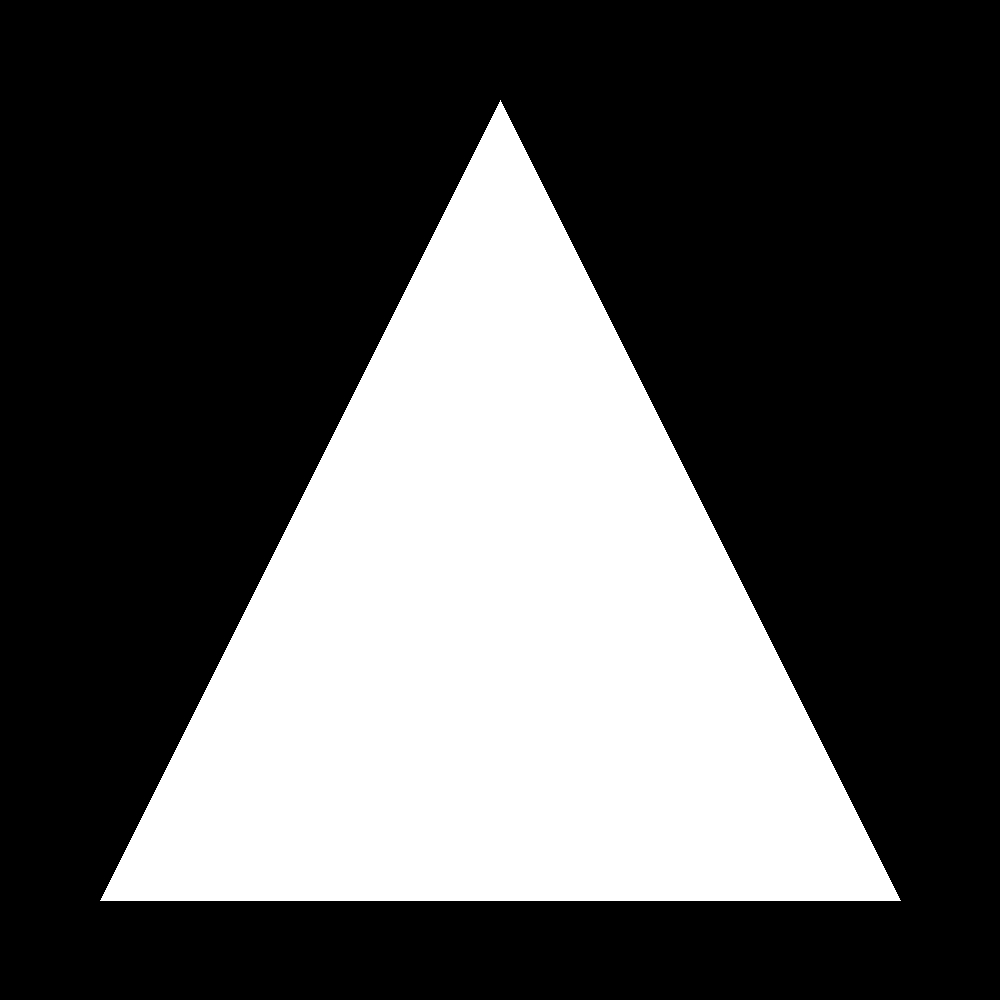
\includegraphics[width=\textwidth]{triangle.png}
		\caption{triangle}
		\label{fig:triangle}
	\end{subfigure}
	\caption{Basic binary shapes generated using the Python \texttt{PIL} library.}
	\label{fig:shapes}
\end{figure}

For extracting the edges of the shapes, I explored a few edge detection algorithms, eventually settling with the following

\begin{itemize}
	\item \textbf{\texttt{PIL}'s \texttt{FIND\_EDGES} filter} -- this built-in function works like a charm and can be easily implemented as a one-liner. The documentation doesn't describe what it does exactly, but after digging through the source code \cite{pil}, it found that it simply convolves an image with a spot kernel of the form
	
	\begin{equation}\label{eq:spot-kernel}
		G = \mqty( -1 & -1 & -1 \\
				   -1 &  8 & -1 \\
			   	   -1 & -1 & -1 )
	\end{equation}
	
	\item \textbf{Sobel filter} -- approximates the gradient of an image's intensity function \cite{sobel}. Convolves images with two kernels (one for each direction)
	
	\begin{equation}\label{eq:sobel-kernel}
		G_x = \mqty( -1 & 0 & 1 \\
			  		 -2 & 0 & 2 \\
			   		 -1 & 0 & 1 )
		,\qquad
		G_y = G_x^\top
	\end{equation}
	
	\item \textbf{Prewitt filter} -- also approximates the gradient of image intensity and acts in two directions, similar to the Sobel filter \cite{prewitt}. Its kernel is of the form
	
	\begin{equation}\label{eq:prewitt-kernel}
		G_x = \mqty( 1 & 0 & -1 \\
			  		 1 & 0 & -1 \\
			   		 1 & 0 & -1 )
		,\qquad
		G_y = G_x^\top
	\end{equation}
	
	\item \textbf{Laplacian filter} -- calculates the second-order derivatives of the image intensity in one pass \citep{medium}. Because of its sensitivity to noise, I first applied a $3\times 3$ Gaussan filter with 0 standard deviation before applying the Laplacian filter. Its kernel is of the form
	
	\begin{equation}\label{eq:laplacian-kernel}
		G = \mqty( 0 & -1 & 0 \\
			  	  -1 &  4 & -1 \\
			   	   0 & -1 & 0 )
	\end{equation}
	
	\item \textbf{Canny filter} -- a multistage edge-detection algorithm which is highly versatile and efficient \cite{canny}.
	
\end{itemize}

From the traced edges, the area it encloses can be calculated using a discretized form of Green's theorem \cite{soriano}:

\begin{equation}\label{eq:green}
	A = \frac{1}{2} \sum_{i=1}^N \qty(x_{i-1}y_i - y_{i-1}x_i)
\end{equation}

\noindent
where $x_i, y_i$ are the pixel coordinates, and $N$ is the number of pixels on the boundary. The results for each algorithm, along with their relative errors, are shown in Table \ref{tab:area}, and the edge-traced images are shown in Figs. \ref{fig:circle-edges}--\ref{fig:triangle-edges}.

\begin{figure}[htb]
    \centering
	\begin{subfigure}[h!]{0.19\textwidth}
		\centering
		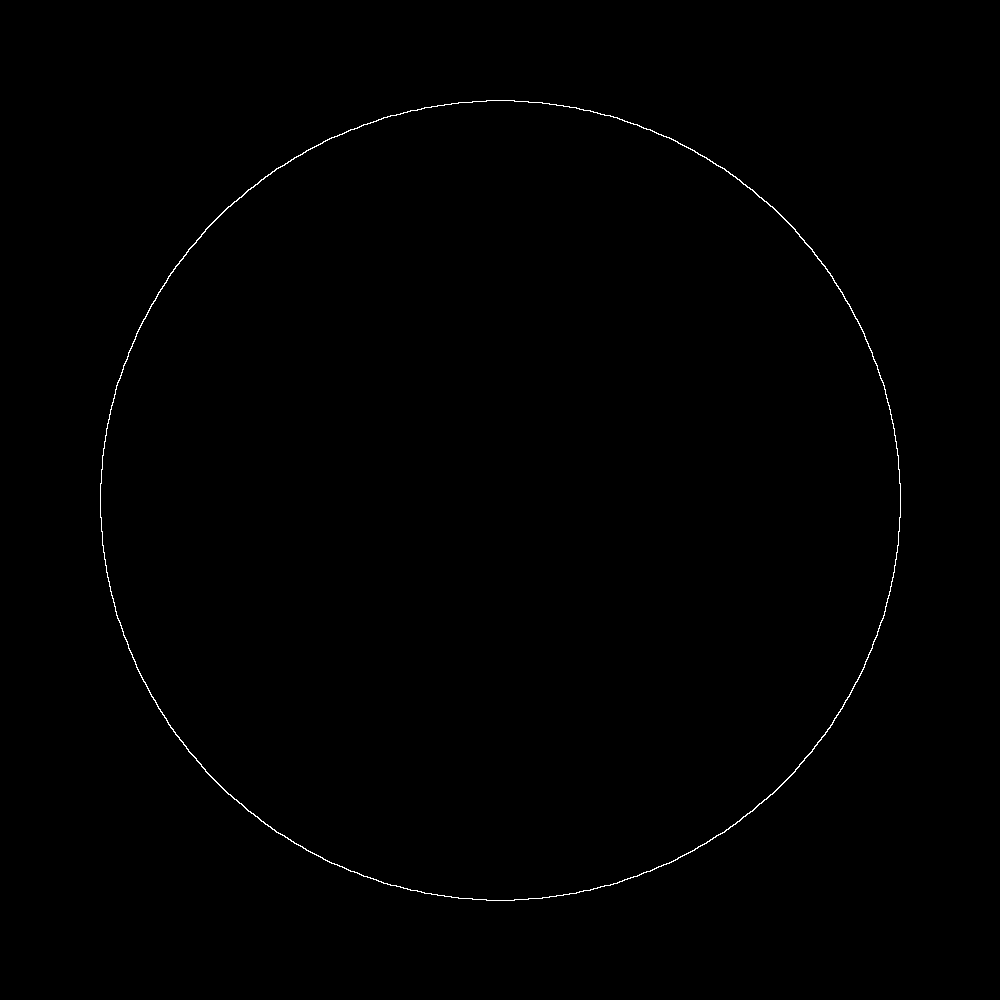
\includegraphics[width=\textwidth]{circle_spot.png}
		\caption{spot}
		\label{fig:circle-spot}
	\end{subfigure}
	\begin{subfigure}[h!]{0.19\textwidth}
		\centering
		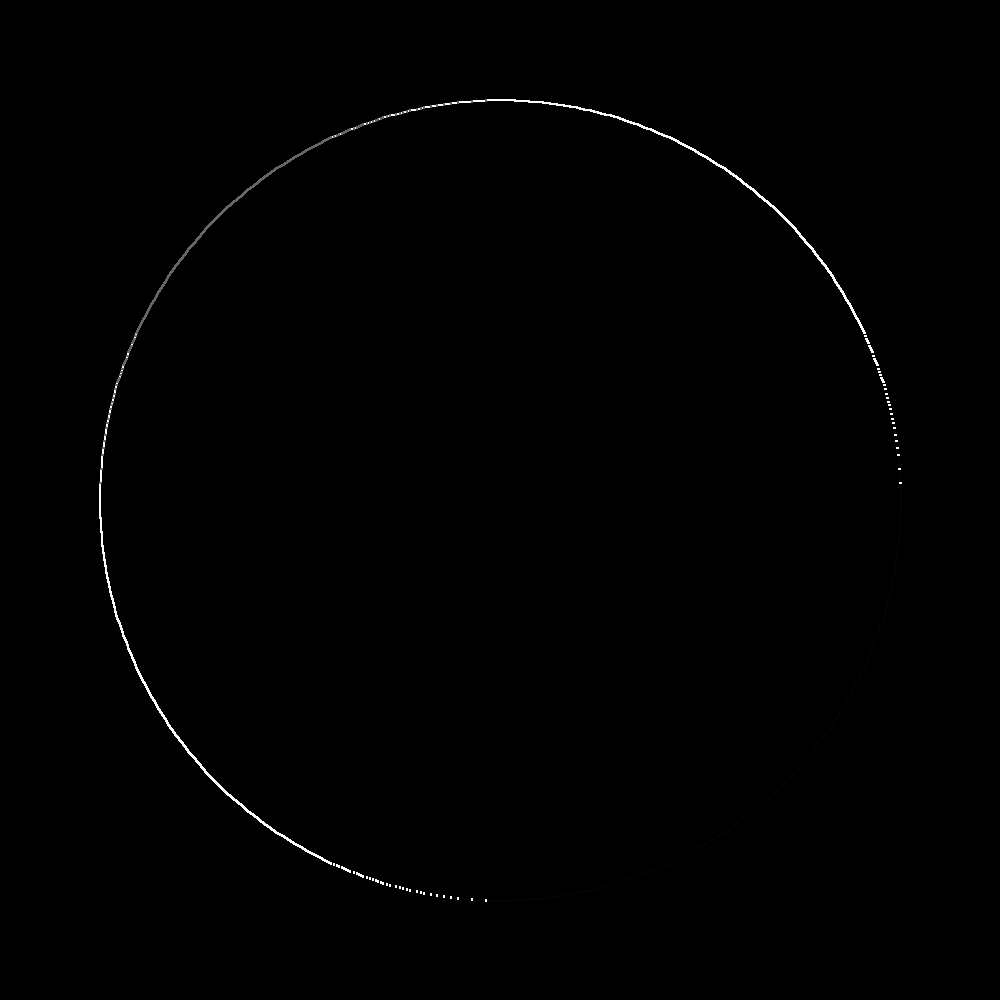
\includegraphics[width=\textwidth]{circle_sobel.png}
		\caption{Sobel}
		\label{fig:cirlce-sobel}
	\end{subfigure}
	\begin{subfigure}[h!]{0.19\textwidth}
		\centering
		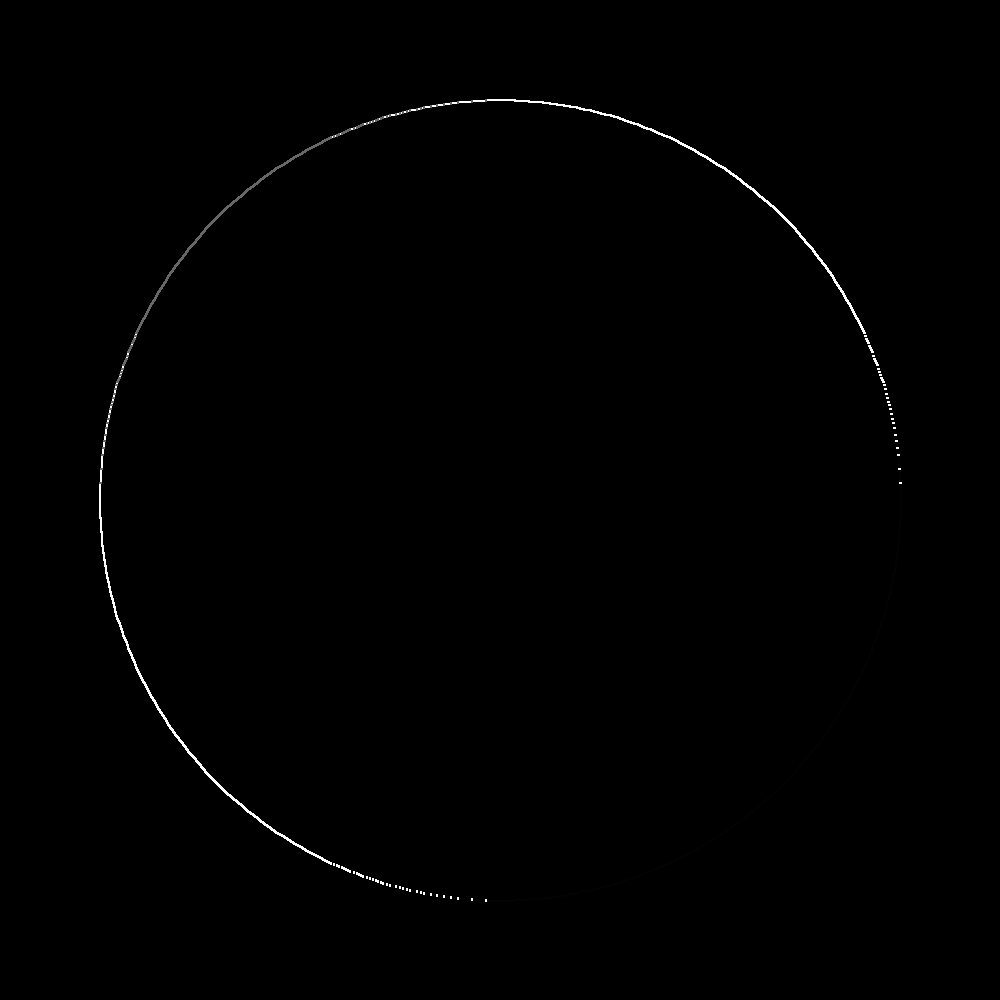
\includegraphics[width=\textwidth]{circle_prewitt.png}
		\caption{Prewitt}
		\label{fig:circle-prewitt}
	\end{subfigure}
	\begin{subfigure}[h!]{0.19\textwidth}
		\centering
		
\includegraphics[width=\textwidth]{circle_laplacian.png}
		\caption{Laplacian}
		\label{fig:circle-laplacian}
	\end{subfigure}
		\begin{subfigure}[h!]{0.19\textwidth}
		\centering
		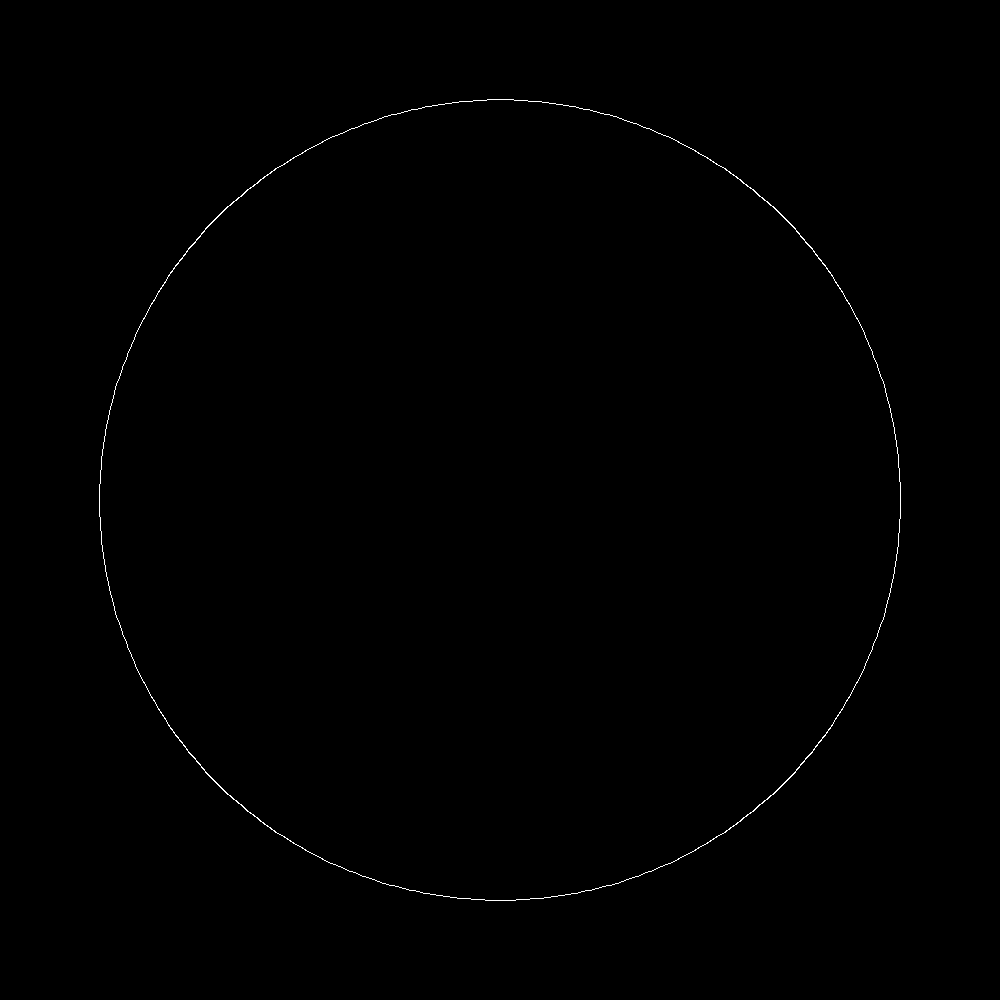
\includegraphics[width=\textwidth]{circle_canny.png}
		\caption{Canny}
		\label{fig:circle-canny}
	\end{subfigure}
	\caption{Edges extracted from the circle using different algorithms.}
	\label{fig:circle-edges}
\end{figure}

\begin{figure}[htb]
    \centering
	\begin{subfigure}[h!]{0.19\textwidth}
		\centering
		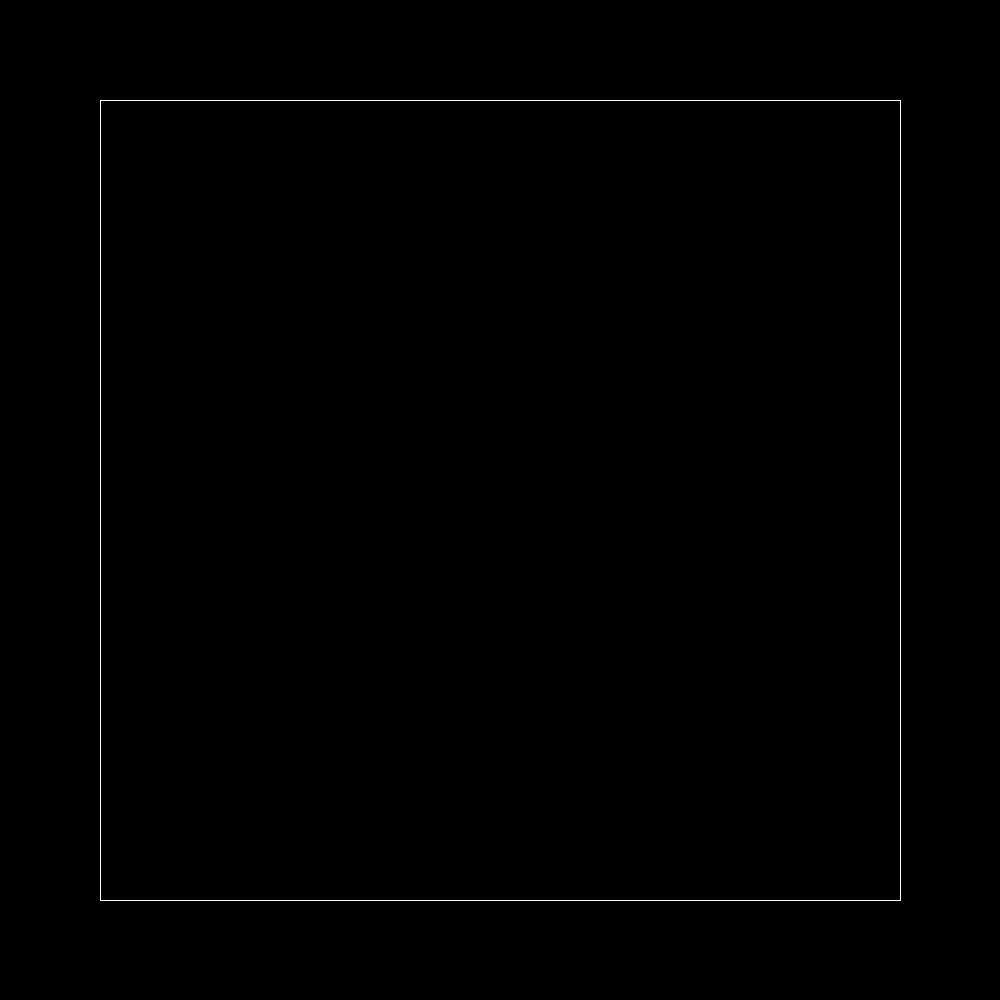
\includegraphics[width=\textwidth]{square_spot.png}
		\caption{spot}
		\label{fig:square-spot}
	\end{subfigure}
	\begin{subfigure}[h!]{0.19\textwidth}
		\centering
		
\includegraphics[width=\textwidth]{square_sobel.png}
		\caption{Sobel}
		\label{fig:square-sobel}
	\end{subfigure}
	\begin{subfigure}[h!]{0.19\textwidth}
		\centering
		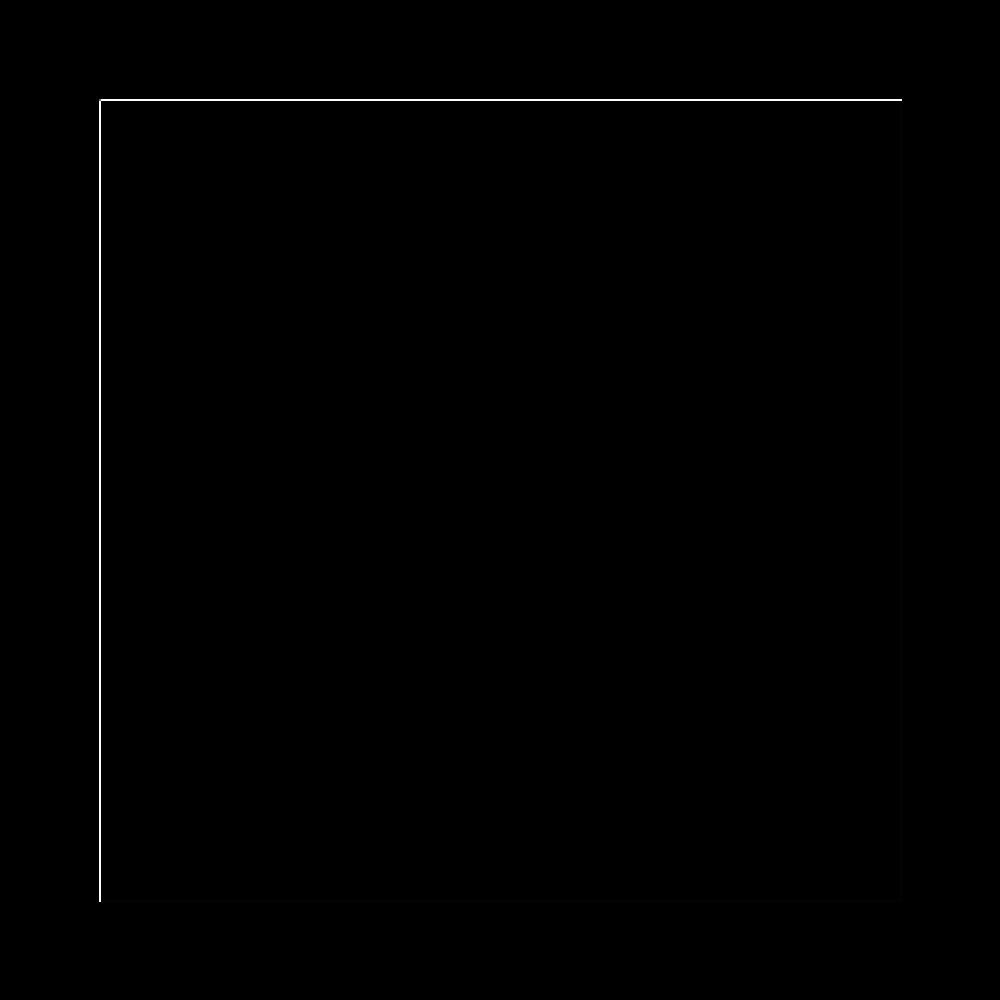
\includegraphics[width=\textwidth]{square_prewitt.png}
		\caption{Prewitt}
		\label{fig:square-prewitt}
	\end{subfigure}
	\begin{subfigure}[h!]{0.19\textwidth}
		\centering
		
\includegraphics[width=\textwidth]{square_laplacian.png}
		\caption{Laplacian}
		\label{fig:square-laplacian}
	\end{subfigure}
		\begin{subfigure}[h!]{0.19\textwidth}
		\centering
		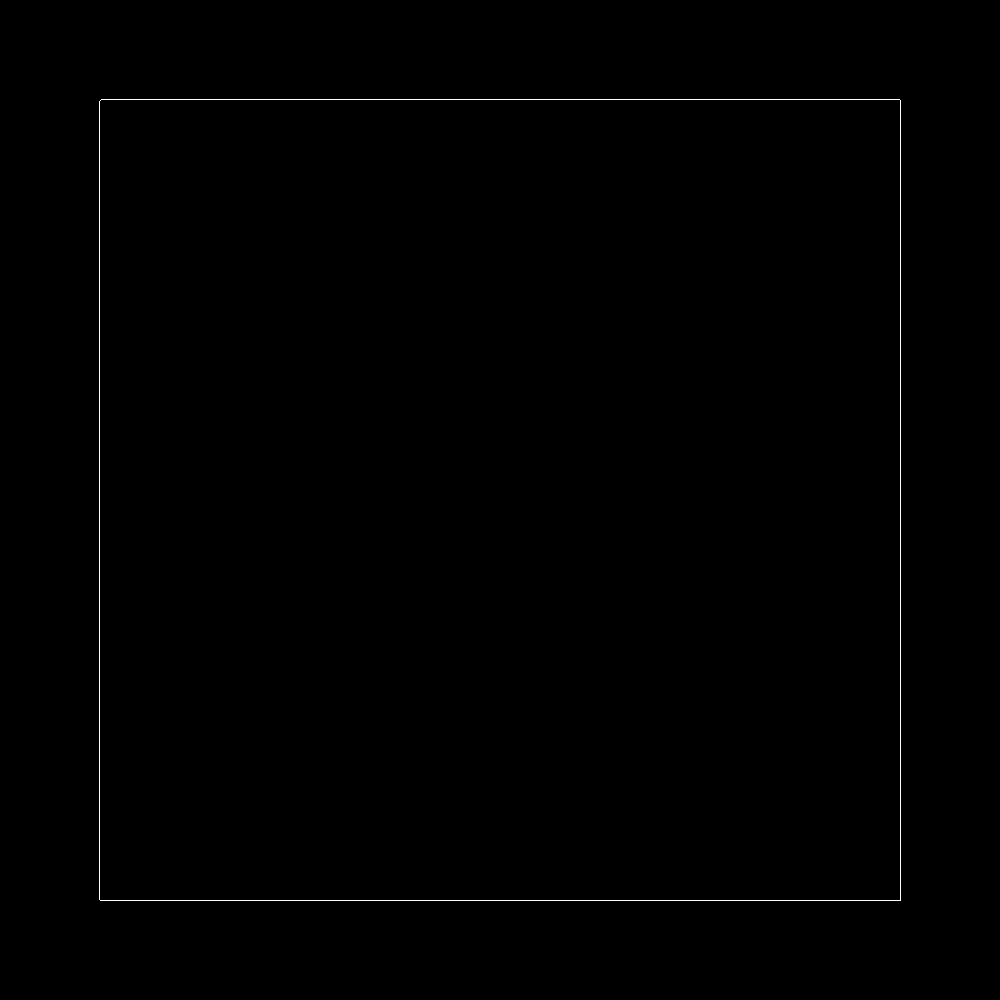
\includegraphics[width=\textwidth]{square_canny.png}
		\caption{Canny}
		\label{fig:square-canny}
	\end{subfigure}
	\caption{Edges extracted from the square using different algorithms.}
	\label{fig:square-edges}
\end{figure}

\begin{figure}[htb]
    \centering
	\begin{subfigure}[h!]{0.19\textwidth}
		\centering
		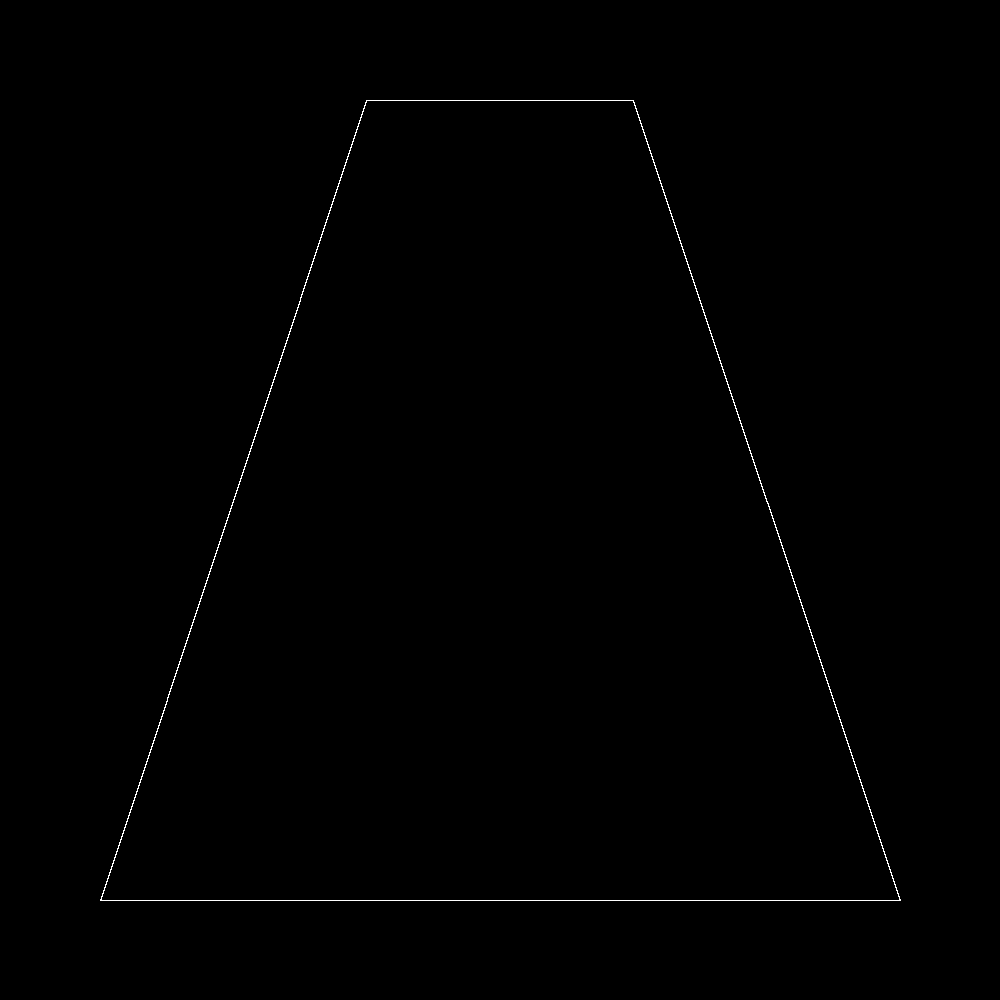
\includegraphics[width=\textwidth]{trapezoid_spot.png}
		\caption{spot}
		\label{fig:trapezoid-spot}
	\end{subfigure}
	\begin{subfigure}[h!]{0.19\textwidth}
		\centering
		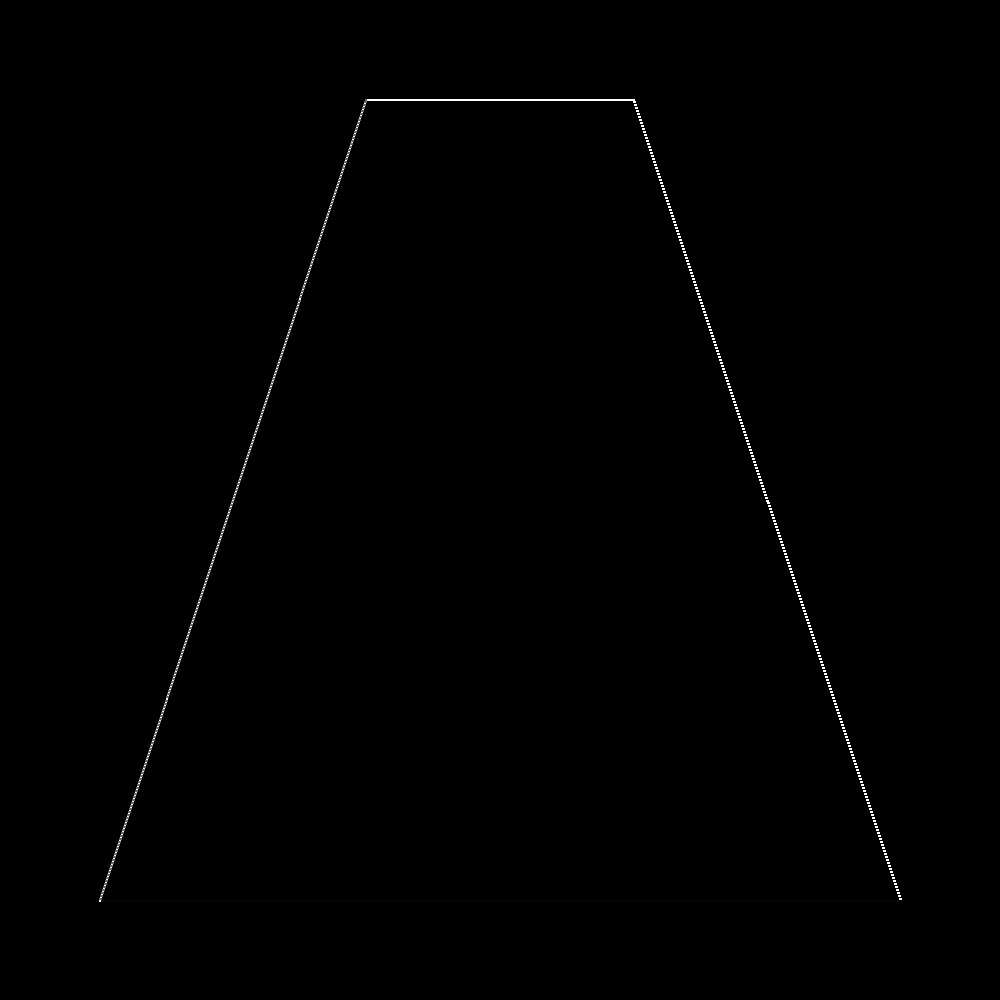
\includegraphics[width=\textwidth]{trapezoid_sobel.png}
		\caption{Sobel}
		\label{fig:trapezoid-sobel}
	\end{subfigure}
	\begin{subfigure}[h!]{0.19\textwidth}
		\centering
		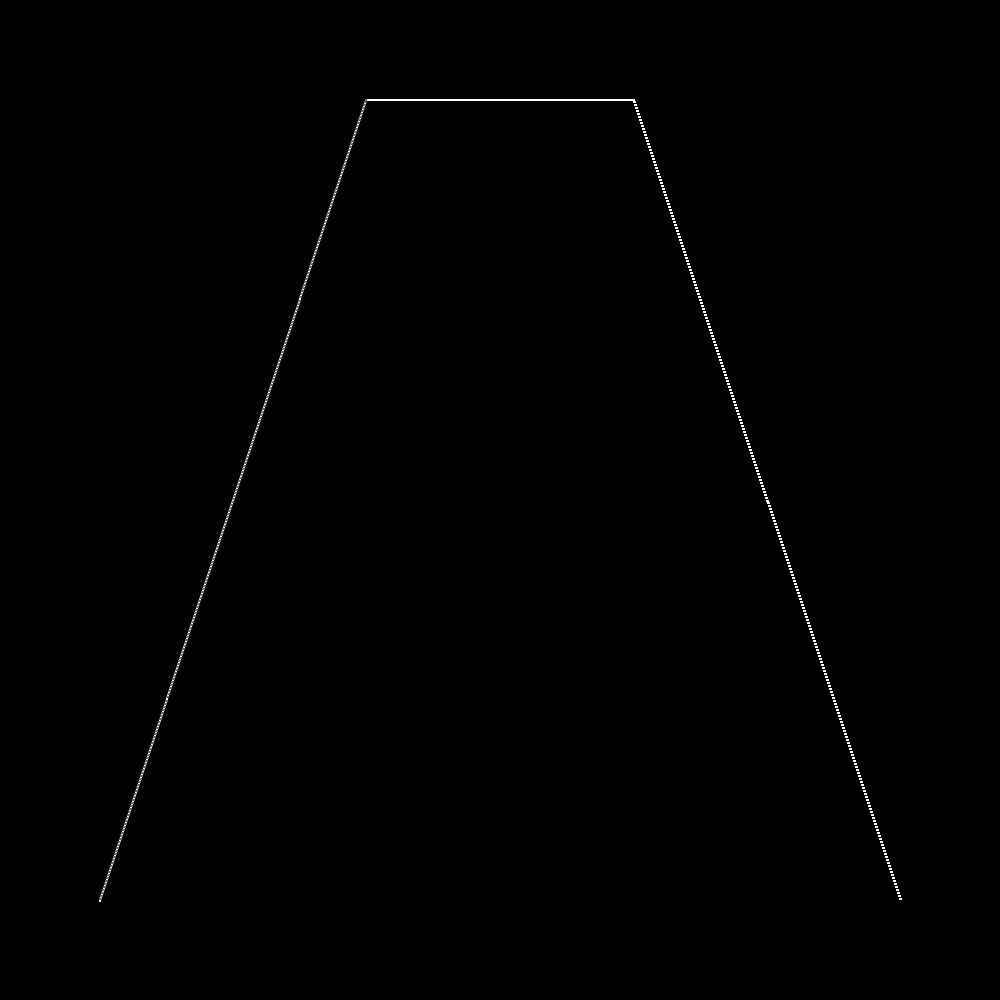
\includegraphics[width=\textwidth]{trapezoid_prewitt.png}
		\caption{Prewitt}
		\label{fig:trapezoid-prewitt}
	\end{subfigure}
	\begin{subfigure}[h!]{0.19\textwidth}
		\centering
		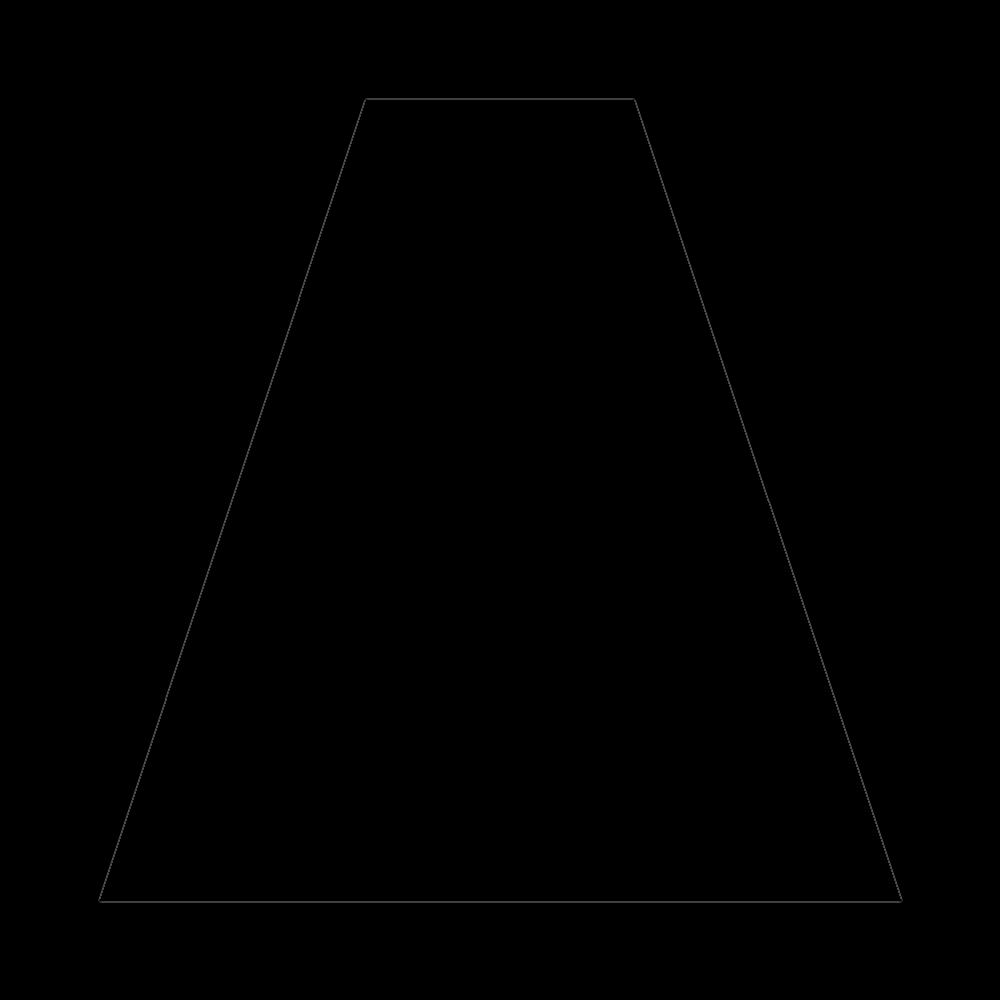
\includegraphics[width=\textwidth]{trapezoid_laplacian.png}
		\caption{Laplacian}
		\label{fig:trapezoid-laplacian}
	\end{subfigure}
		\begin{subfigure}[h!]{0.19\textwidth}
		\centering
		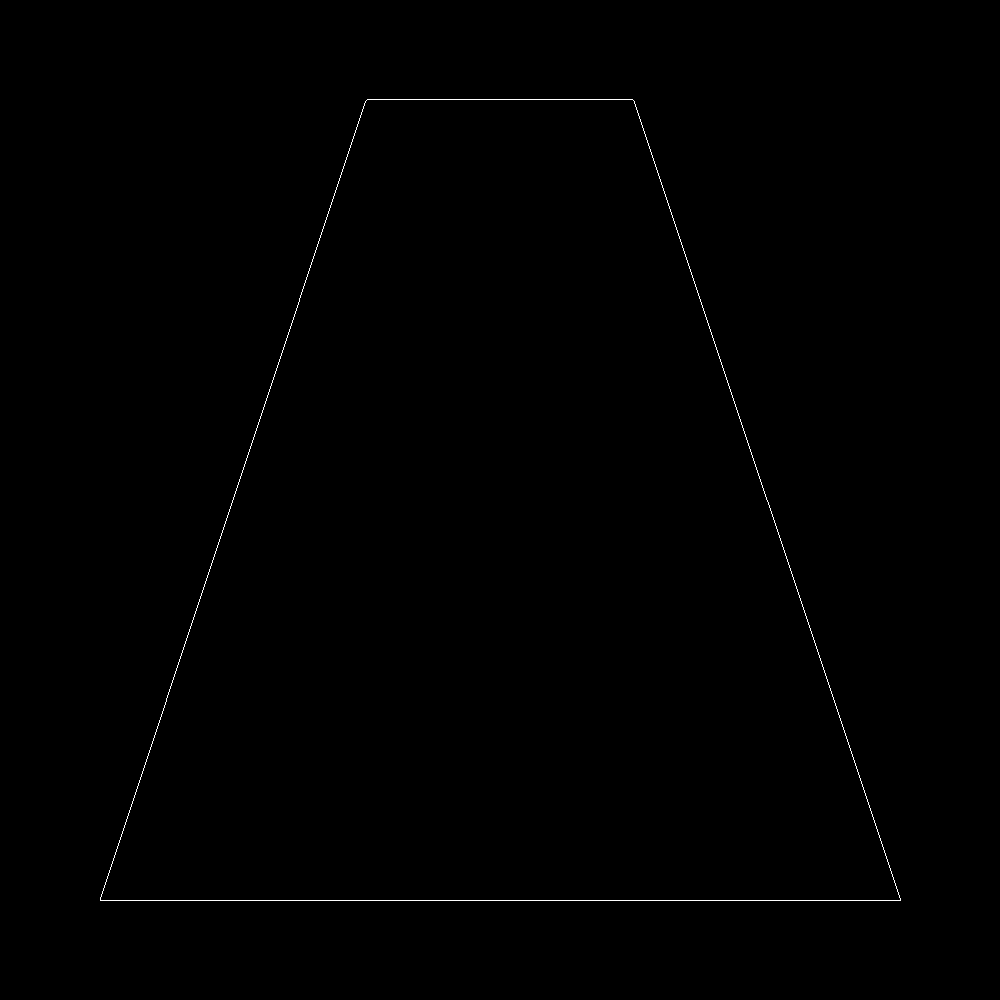
\includegraphics[width=\textwidth]{trapezoid_canny.png}
		\caption{Canny}
		\label{fig:trapezoid-canny}
	\end{subfigure}
	\caption{Edges extracted from the trapezoid using different algorithms.}
	\label{fig:trapezoid-edges}
\end{figure}

\begin{figure}[htb]
    \centering
	\begin{subfigure}[h!]{0.19\textwidth}
		\centering
		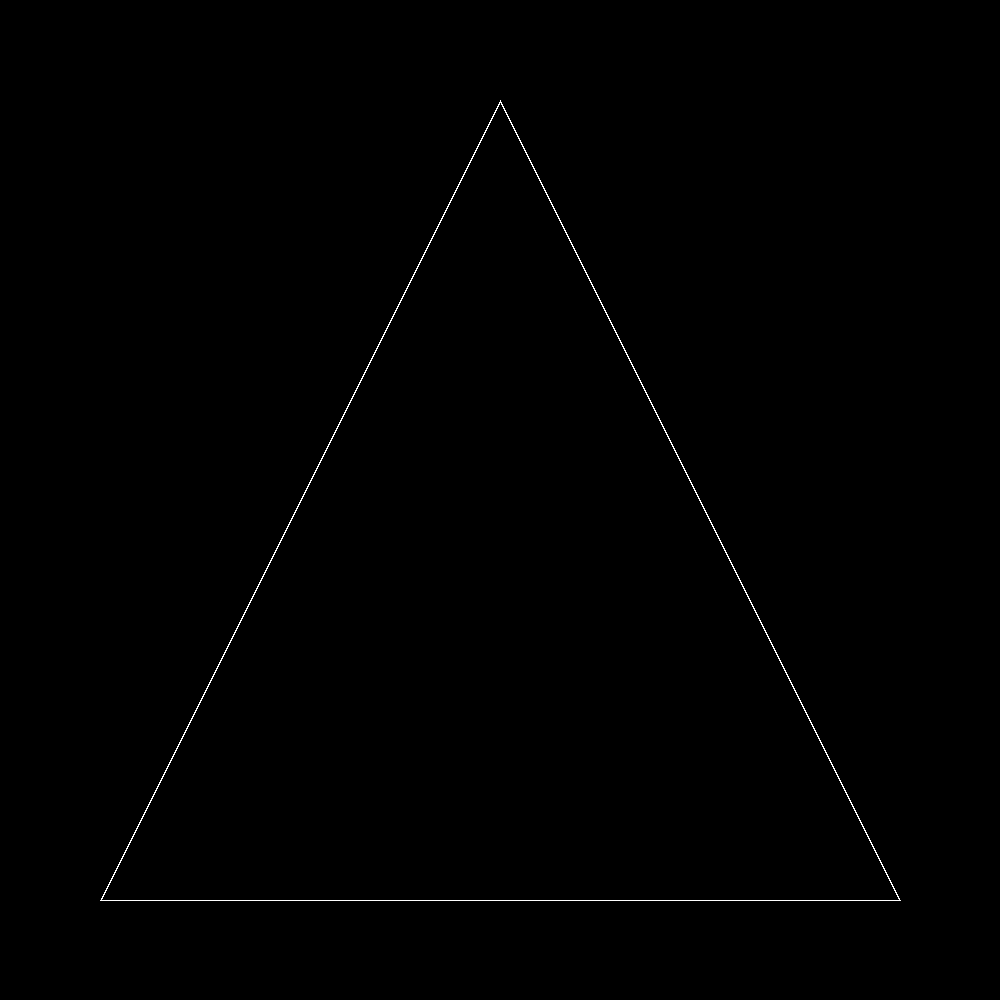
\includegraphics[width=\textwidth]{triangle_spot.png}
		\caption{spot}
		\label{fig:triangle-spot}
	\end{subfigure}
	\begin{subfigure}[h!]{0.19\textwidth}
		\centering
		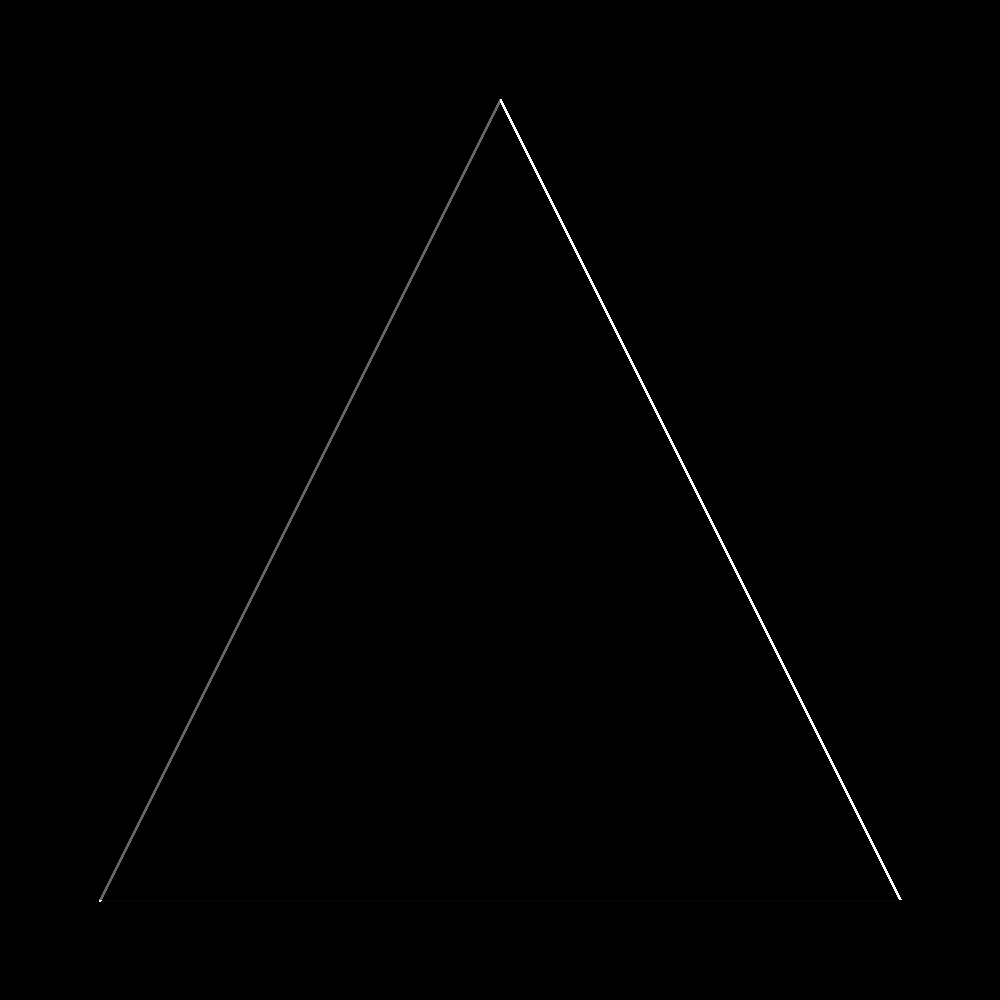
\includegraphics[width=\textwidth]{triangle_sobel.png}
		\caption{Sobel}
		\label{fig:triangle-sobel}
	\end{subfigure}
	\begin{subfigure}[h!]{0.19\textwidth}
		\centering
		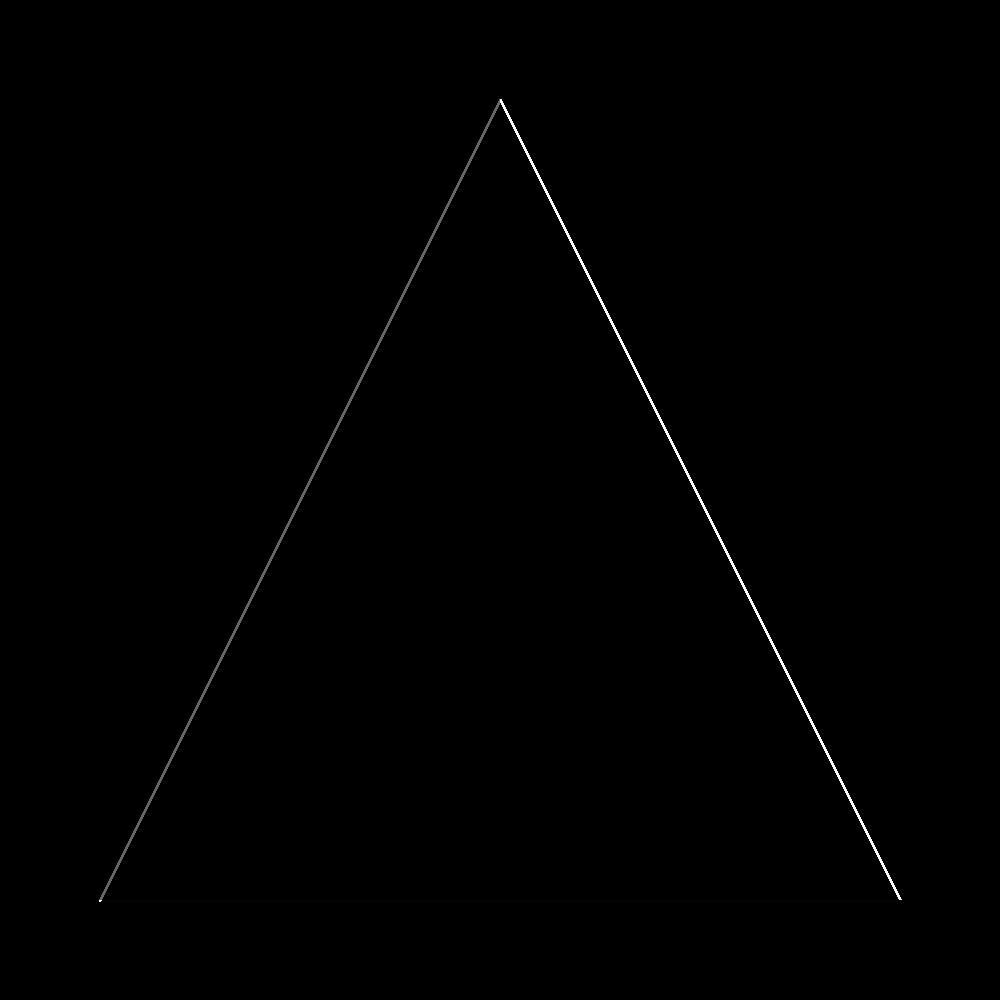
\includegraphics[width=\textwidth]{triangle_prewitt.png}
		\caption{Prewitt}
		\label{fig:triangle-prewitt}
	\end{subfigure}
	\begin{subfigure}[h!]{0.19\textwidth}
		\centering
		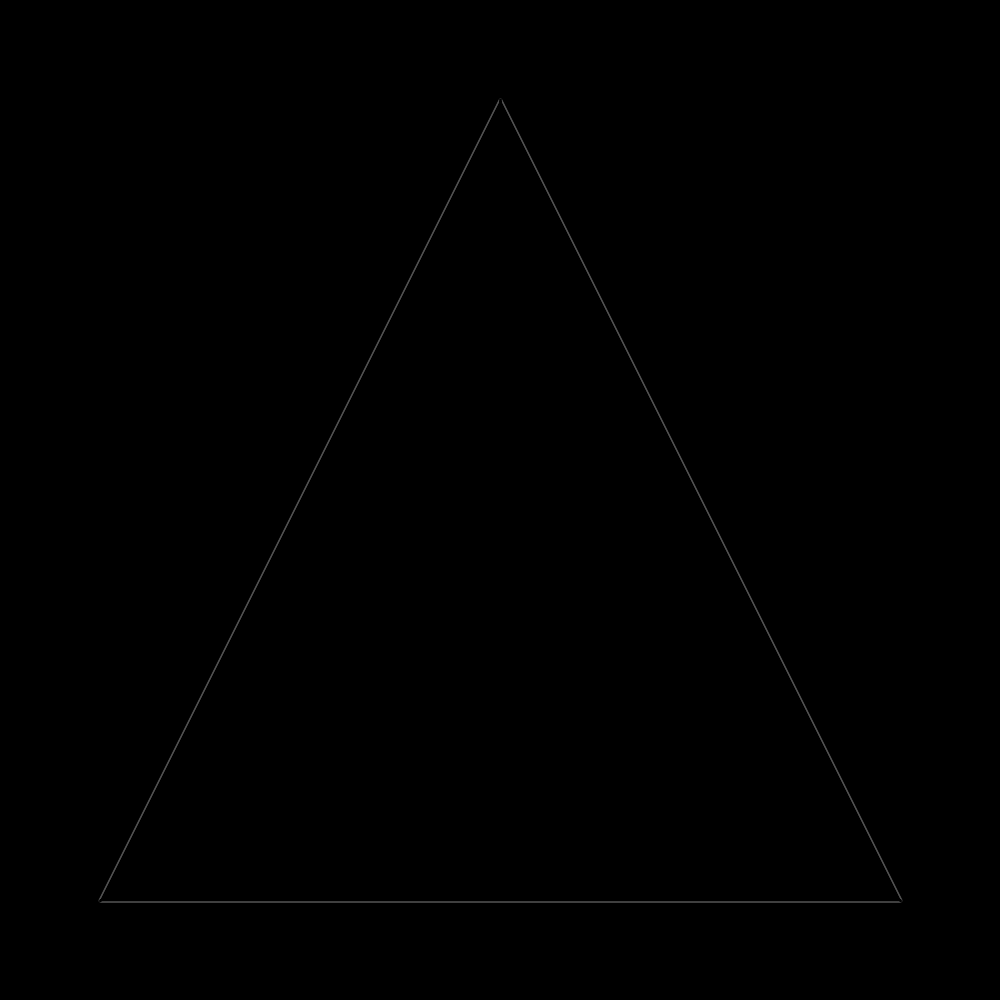
\includegraphics[width=\textwidth]{triangle_laplacian.png}
		\caption{Laplacian}
		\label{fig:triangle-laplacian}
	\end{subfigure}
		\begin{subfigure}[h!]{0.19\textwidth}
		\centering
		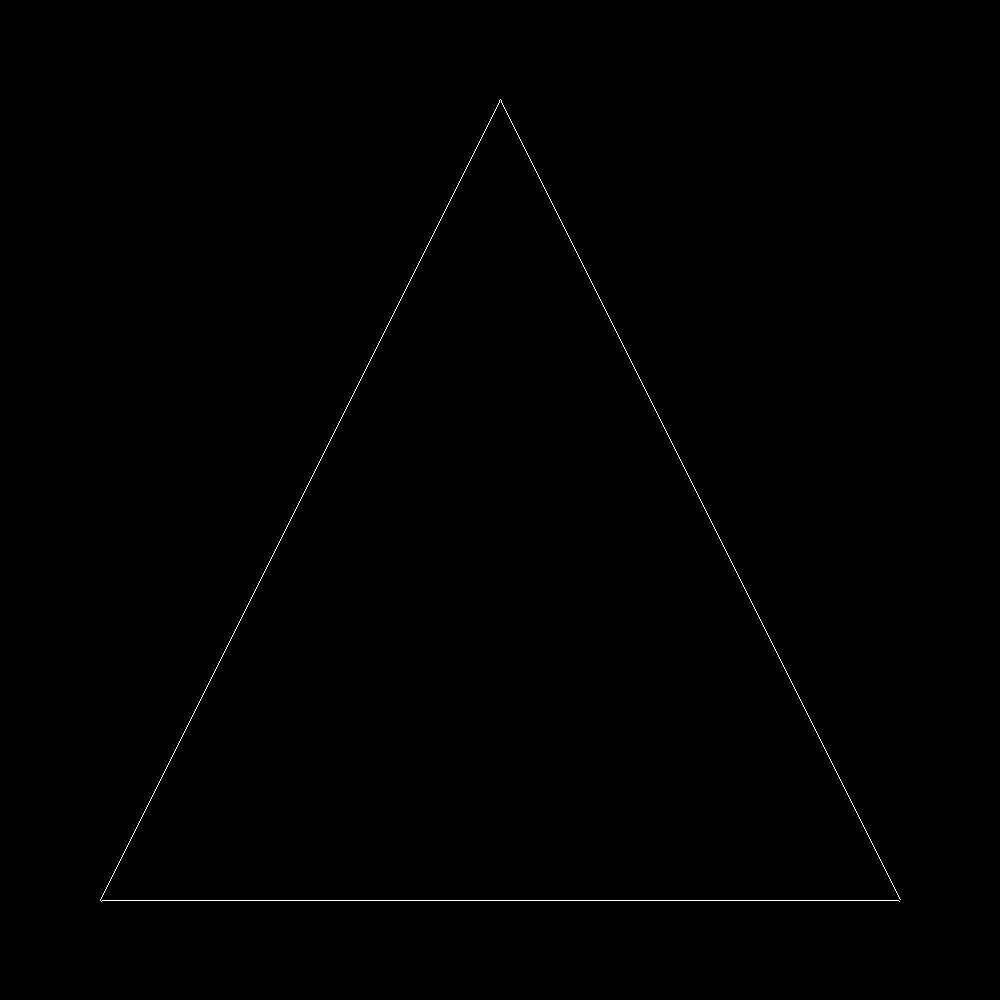
\includegraphics[width=\textwidth]{triangle_canny.png}
		\caption{Canny}
		\label{fig:triangle-canny}
	\end{subfigure}
	\caption{Edges extracted from the triangle using different algorithms.}
	\label{fig:triangle-edges}
\end{figure}

Notice how the Sobel \& Prewitt filters perform very similarly because they are both gradient-based methods. Due to their directional dependence, we can notice how the edges, particularly on the lower-right portions, are not being detected very well. Upon closer examination, however, the edges \textit{are} being detected but are very faint (low magnitude). Spot and Canny, on the other hand, produce very clean and accurate edges. Laplacian also detects a clean edge but is somewhat low in magnitude.

\definecolor{Gray}{gray}{0.9}
\begin{table}[!htb]
	\centering
	\caption{Actual and calculated areas (px$^2$) of each shape and their corresponding relative errors. The percentages in bold indicate the best-performing algorithm for each shape.}
	\begin{tabular}{|c|c|c|c|c|c|c|c|}
		\hline
		Shape & Actual & Spot & Sobel & Prewitt & Laplacian & Canny \\ \hline \hline
		circle & 502,655 & 501,584 & 503,187 & 503,187 & 503,198 & 503,182 \\ \hline
		\rowcolor{Gray}
		& & 0.21\% & 0.11\% & 0.11\% & 0.11\% & \textbf{0.10\%} \\ \hline
		square & 640,000 & 639,800 & 641,404 & 641,404 & 641,416 & 641,398 \\ \hline
		\rowcolor{Gray}
		& & \textbf{0.03\%} & 0.22\% & 0.22\% & 0.22\% & 0.22\% \\ \hline
		trapezoid & 426,667 & 426,399 & 428,002 & 428,002 & 428,013 & 427,731 \\ \hline
		\rowcolor{Gray}
		& & \textbf{0.06\%} & 0.31\% & 0.31\% & 0.32\% & 0.25\% \\ \hline
		triangle & 320,000 & 319,102 & 320,705 & 320,705 & 320,714 & 320,304 \\ \hline
		\rowcolor{Gray}
		& & 0.28\% & 0.22\% & 0.22\% & 0.22\% & \textbf{0.09\%} \\ \hline
	\end{tabular}
	\label{tab:area}
\end{table}

I chose the CS Amphitheater as a location of interest for calculating the area on a map. I obtained its actual area using Google Earth's Ruler tool, then proceeded to import it into Photoshop. I then applied enough threshold so that the yellow line was clear and isolated from the other white spots. I manually erased any remaining white artifacts until only the circle and the line indicating the radius were left. I then measured the length of the radius in pixels, this time using Photoshop's Ruler tool. Since the actual radius in meters was also provided by Google Earth's Ruler tool, I was able to formulate the pixel-to-meter conversion as follows:

\begin{equation}\label{eq:pixel-to-meter}
	x_{\textrm{m}} = x_{\textrm{px}} \times \frac{37.62 \textrm{ m}}{389\textrm{ px}}
\end{equation}

Via Green's theorem, I was able to obtain the Amphitheater's area in pixels. However, this cannot be converted directly to real units using \eqref{eq:pixel-to-meter} because our current units are area, while the conversion equation only works for units of length. Since the amphitheater appears fairly circular, I used the formula for the area of a circle $A = \pi r^2$ and solved for $r$. I can now plug in this $r$ directly into \eqref{eq:pixel-to-meter} and finally, multiply it again by $\pi r$ to get the area in real units. The calculated areas for the different algorithms are shown in Table \ref{tab:amphi-area}, and the edge-traced images are shown in Fig. \ref{fig:csamphi}.

\begin{table}[!htb]
	\centering
	\caption{Actual and calculated areas (m$^2$) of the CS Amphitheater using different algorithms and their corresponding relative errors.}
	\begin{tabular}{|c|c|c|c|c|c|c|}
		\hline
		Actual & Spot & Sobel & Prewitt & Laplacian & Canny \\ \hline \hline
		4485.92 & 4600.44 & 4630.52 & 4630.55 & 4629.64 & 4634.90 \\ \hline
		\rowcolor{Gray}
		& \textbf{2.55\%} & 3.22\% & 3.22\% & 3.20\% & 3.32\% \\ \hline
	\end{tabular}
	\label{tab:amphi-area}
\end{table}

\begin{figure}[htb]
    \centering
	\begin{subfigure}[h!]{0.45\textwidth}
		\centering
		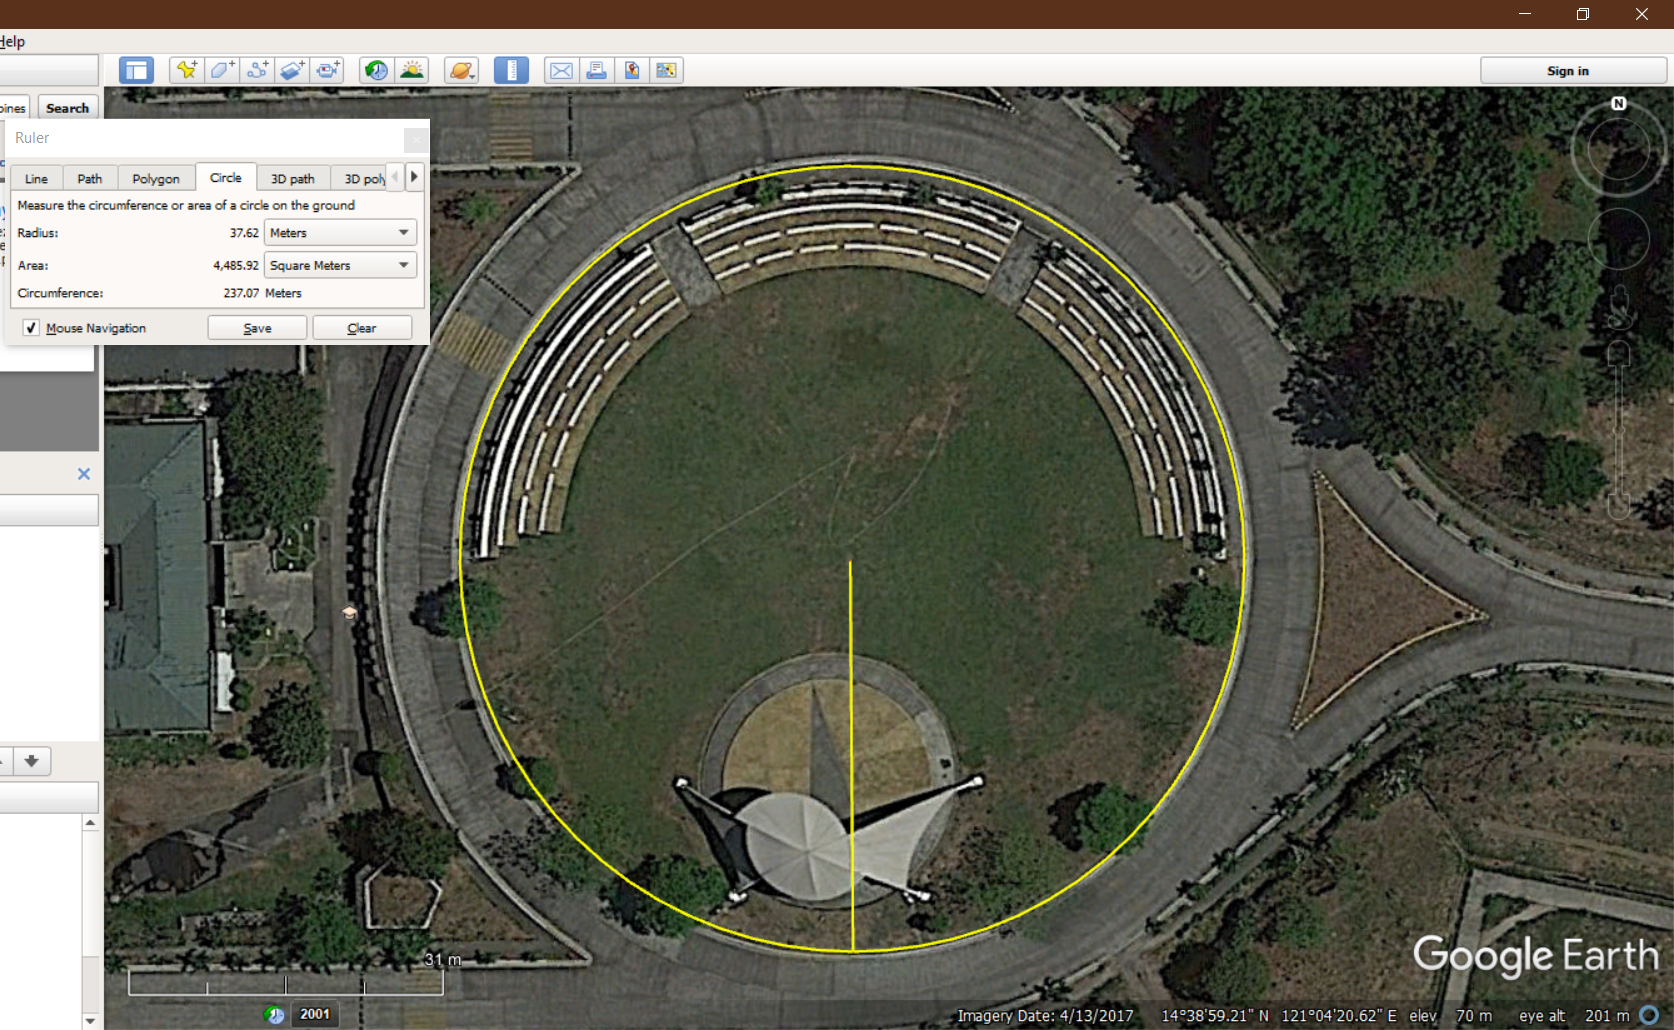
\includegraphics[width=\textwidth]{csamphi_map.png}
		\caption{Enclosed area in Google Earth.}
		\label{fig:amphi-map}
	\end{subfigure}
	\begin{subfigure}[h!]{0.49\textwidth}
		\centering
		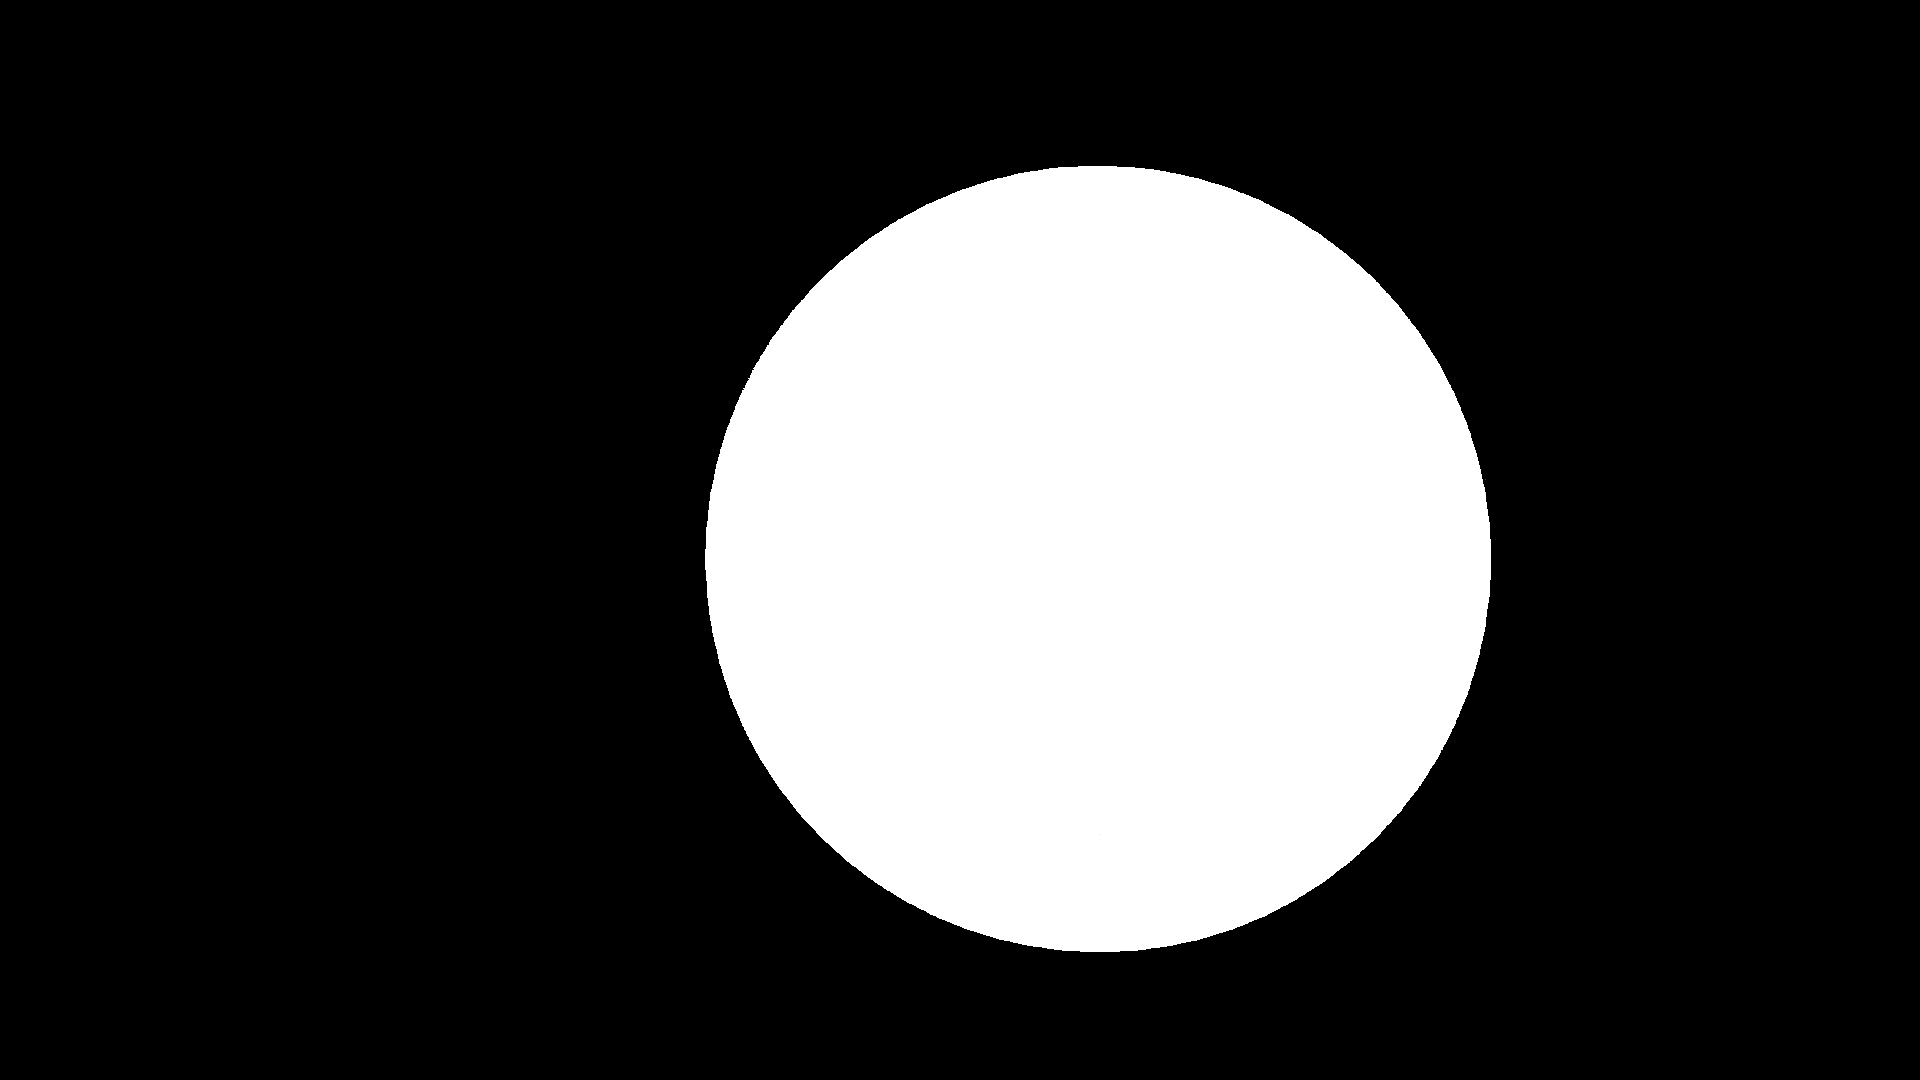
\includegraphics[width=\textwidth]{csamphi.png}
		\caption{Applying threshold and isolating the ROI.}
		\label{fig:amphi}
	\end{subfigure}
	\begin{subfigure}[h!]{0.49\textwidth}
		\centering
		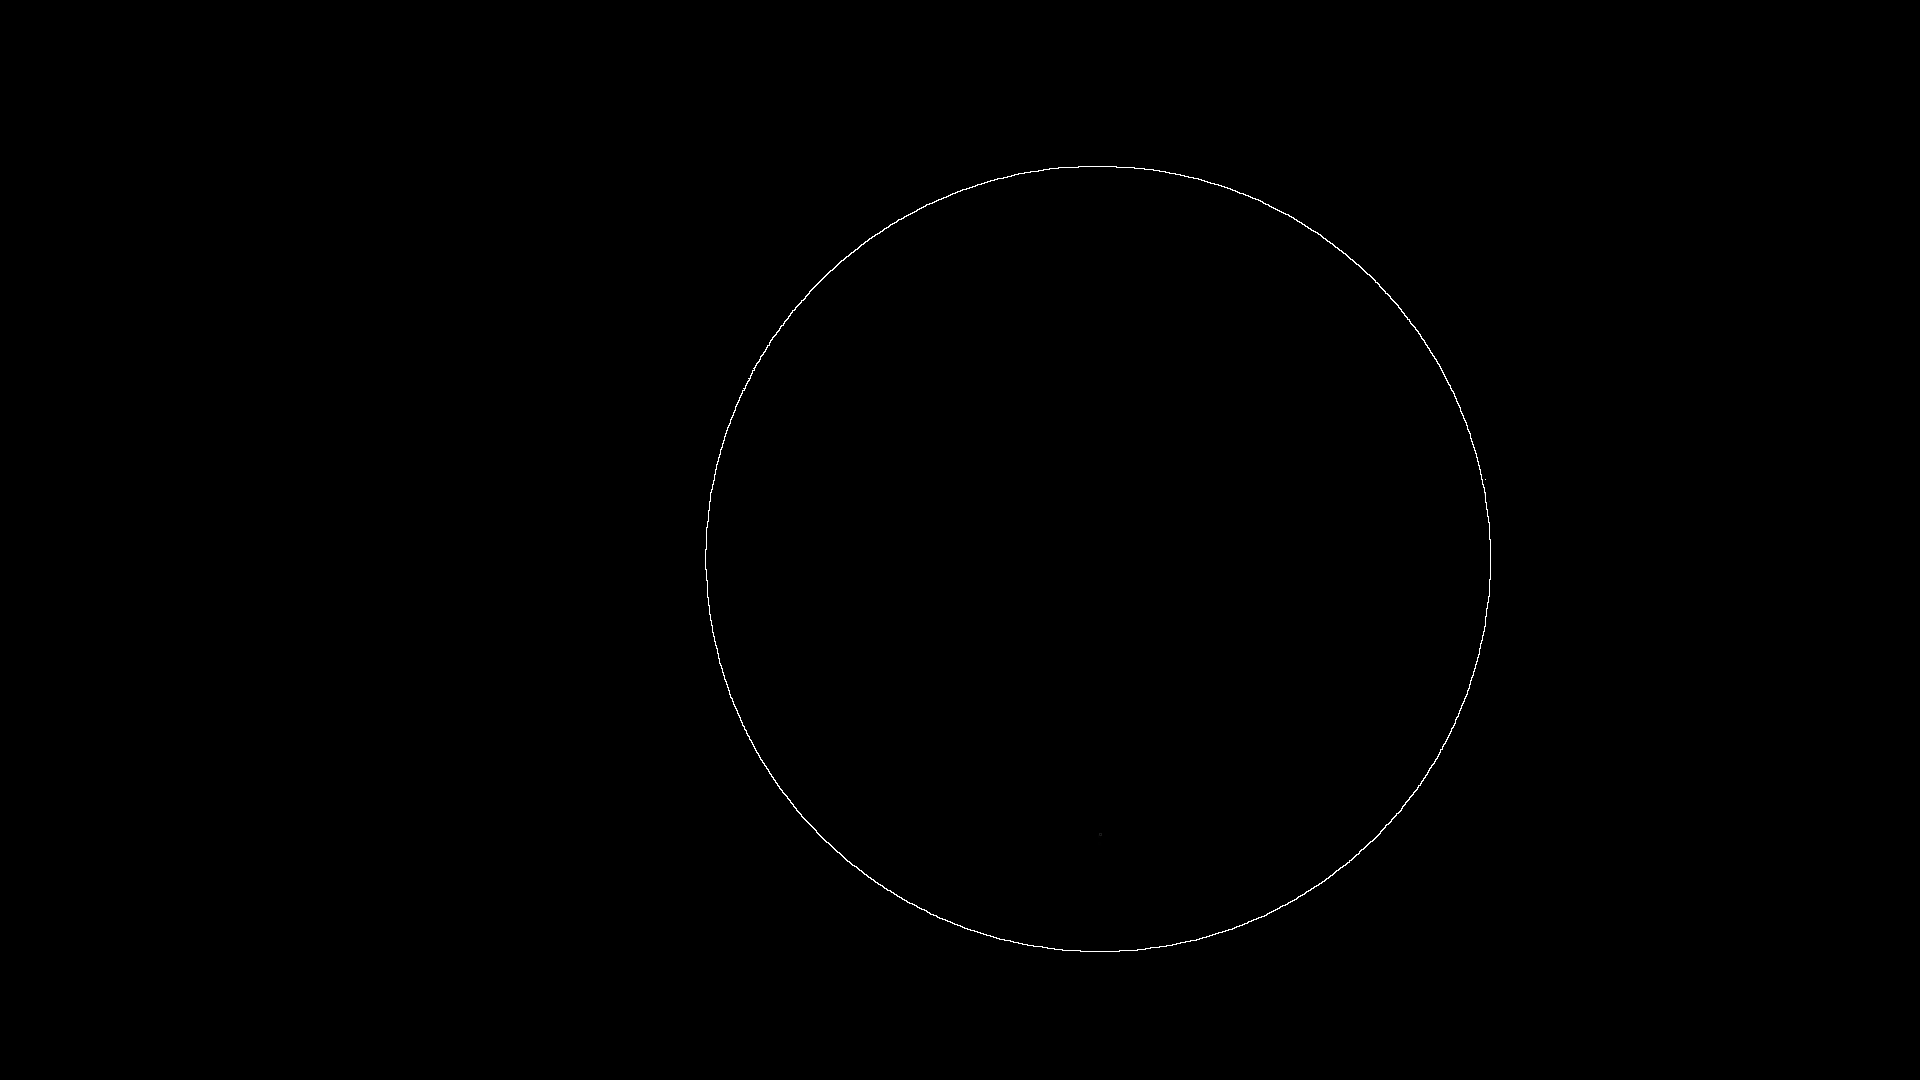
\includegraphics[width=\textwidth]{csamphi_spot.png}
		\caption{spot}
		\label{fig:amphi-spot}
	\end{subfigure}
	\begin{subfigure}[h!]{0.49\textwidth}
		\centering
		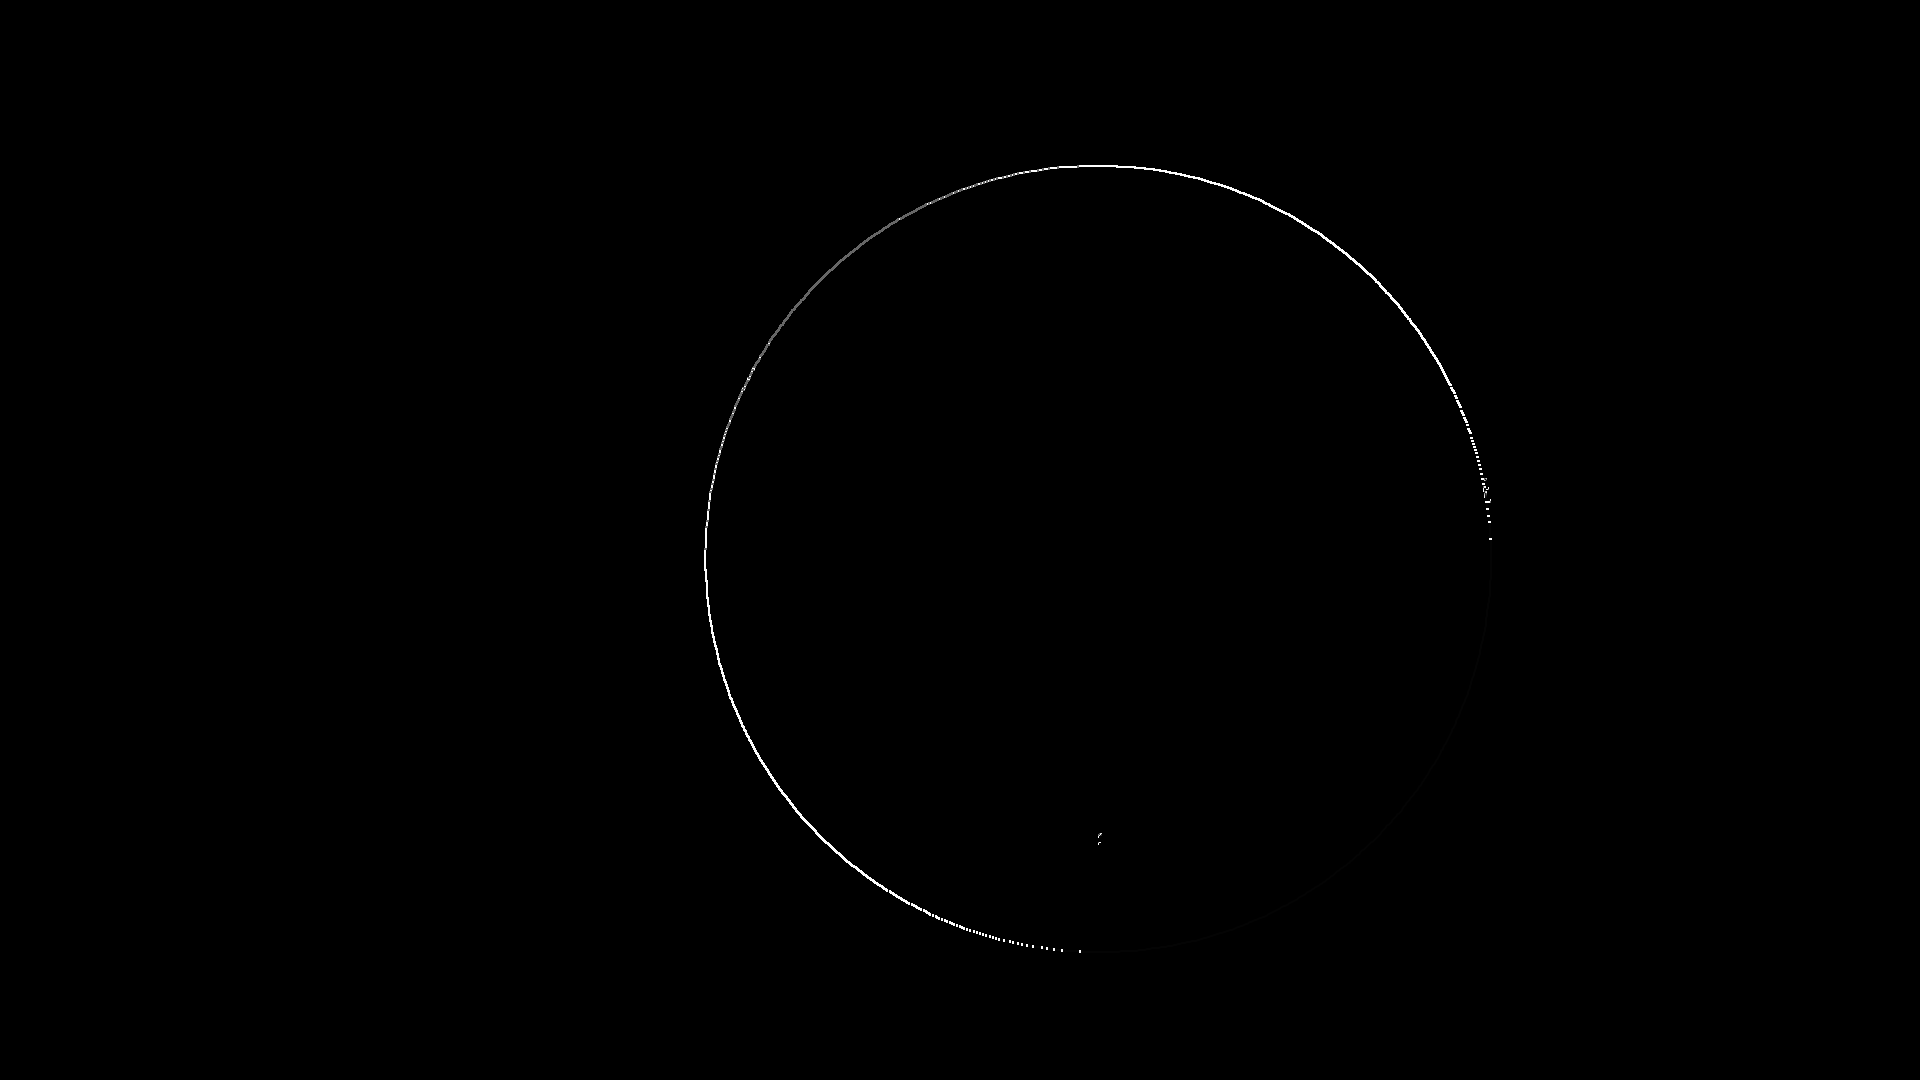
\includegraphics[width=\textwidth]{csamphi_sobel.png}
		\caption{Sobel/Prewitt}
		\label{fig:amphi-sobel}
	\end{subfigure}
	\begin{subfigure}[h!]{0.49\textwidth}
		\centering
		
\includegraphics[width=\textwidth]{csamphi_laplacian.png}
		\caption{Laplacian}
		\label{fig:amphi-laplacian}
	\end{subfigure}
	\begin{subfigure}[h!]{0.49\textwidth}
		\centering
		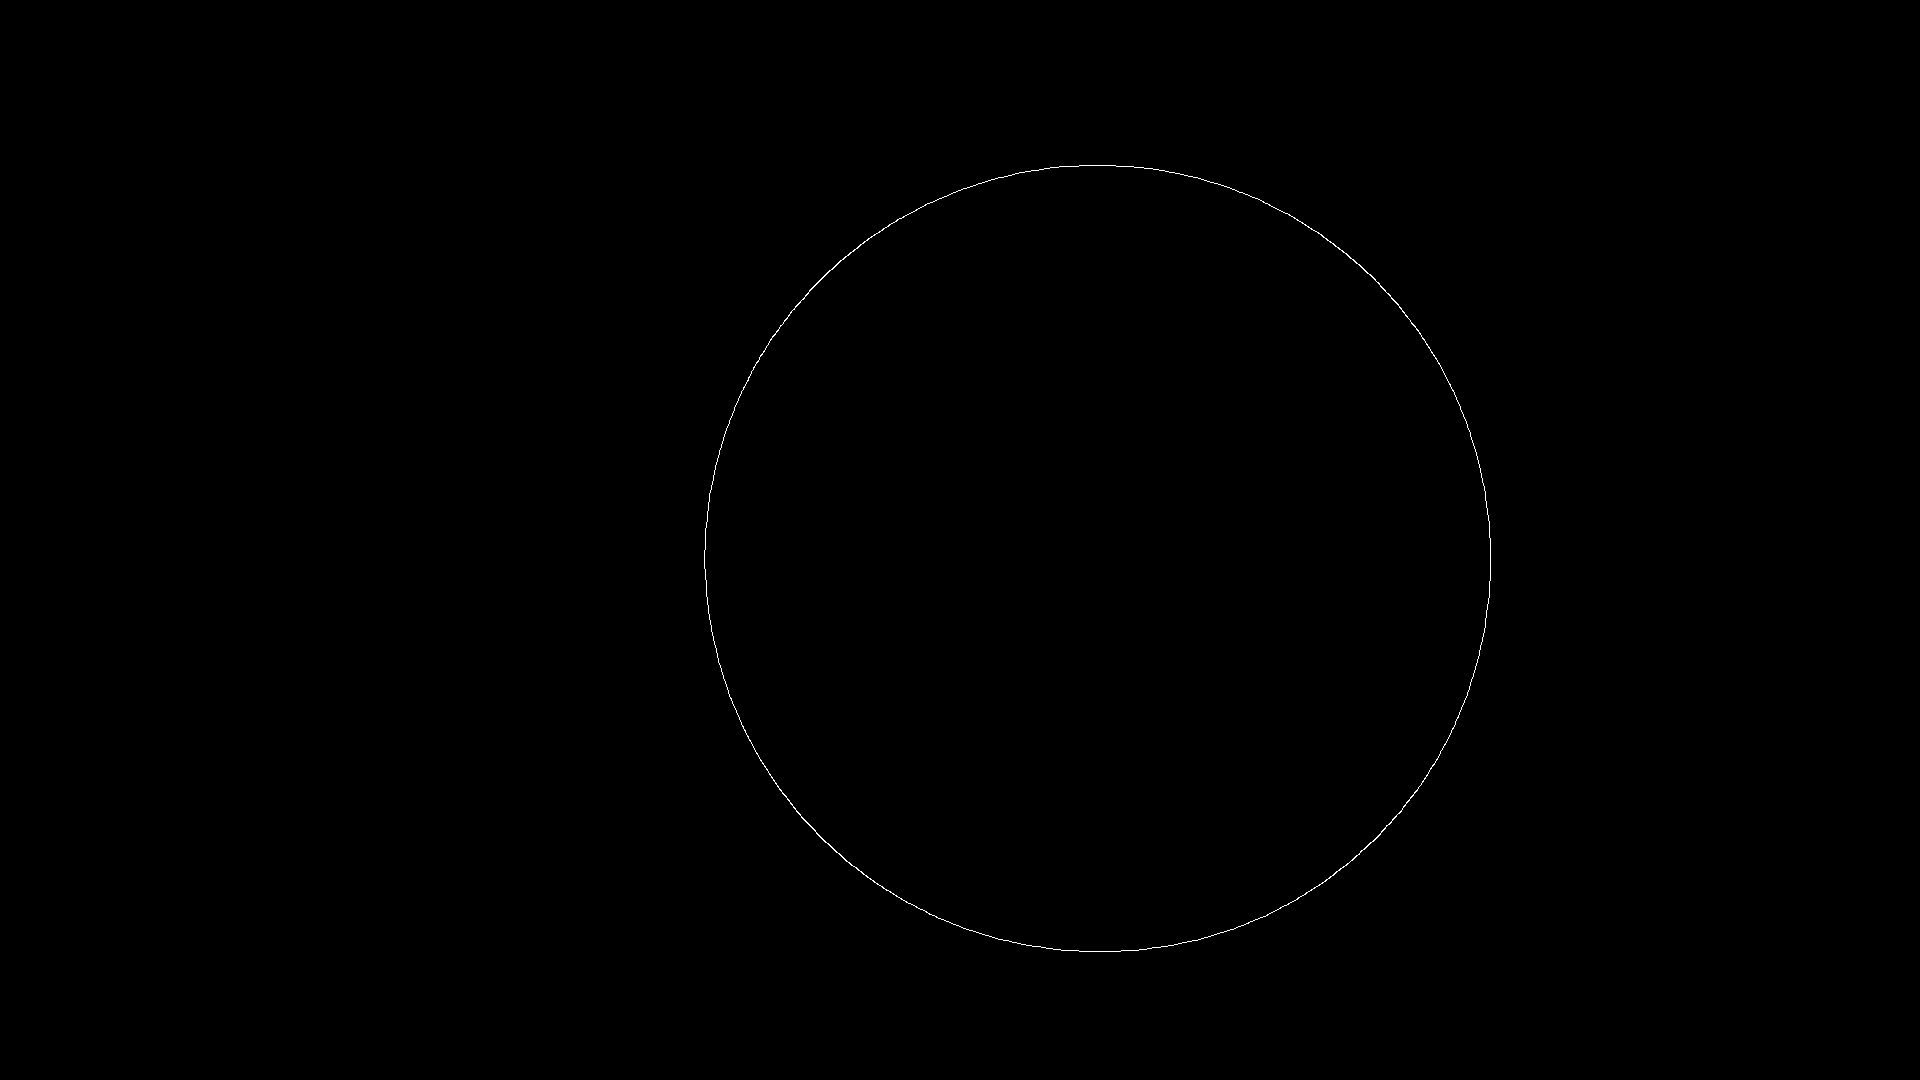
\includegraphics[width=\textwidth]{csamphi_canny.png}
		\caption{Canny}
		\label{fig:amphi-canny}
	\end{subfigure}
	\caption{Detecting the edges of the CS Amphitheater.}
	\label{fig:csamphi}
\end{figure}

\begin{table}[!htb]
	\centering
	\caption{Self-evaluation.}
	\begin{tabular}{|r|c|}
		\hline
		Technical correctness & 5 \\ \hline
		Quality of presentation & 5 \\ \hline
		Initiative & 2 \\ \hline
		\textbf{TOTAL} & \textbf{12} \\ \hline
	\end{tabular}
	\label{tab:self-eval}
\end{table}

We can observe that in general, the spot filter works best in edge detection. Upon further investigation, I found out that the spot kernel is actually a variant of the Laplacian kernel and produces exceptional results on arbitrary images.

\bibliographystyle{spp-bst}
\bibliography{186-Act4}

\end{document}